\section{Definition of filters to select states and topologies }
 
A selector is a mask describing the rules that an entity has to pass in order to be used or rejected. This selector is built of different components, carrying state features. The components can be bound together or not. In a population-based model, the selector, when applied to a pool of entities, permits to filter it, and to obtain a further, more refined, entity pool.

\begin{figure}[H]
\begin{center}
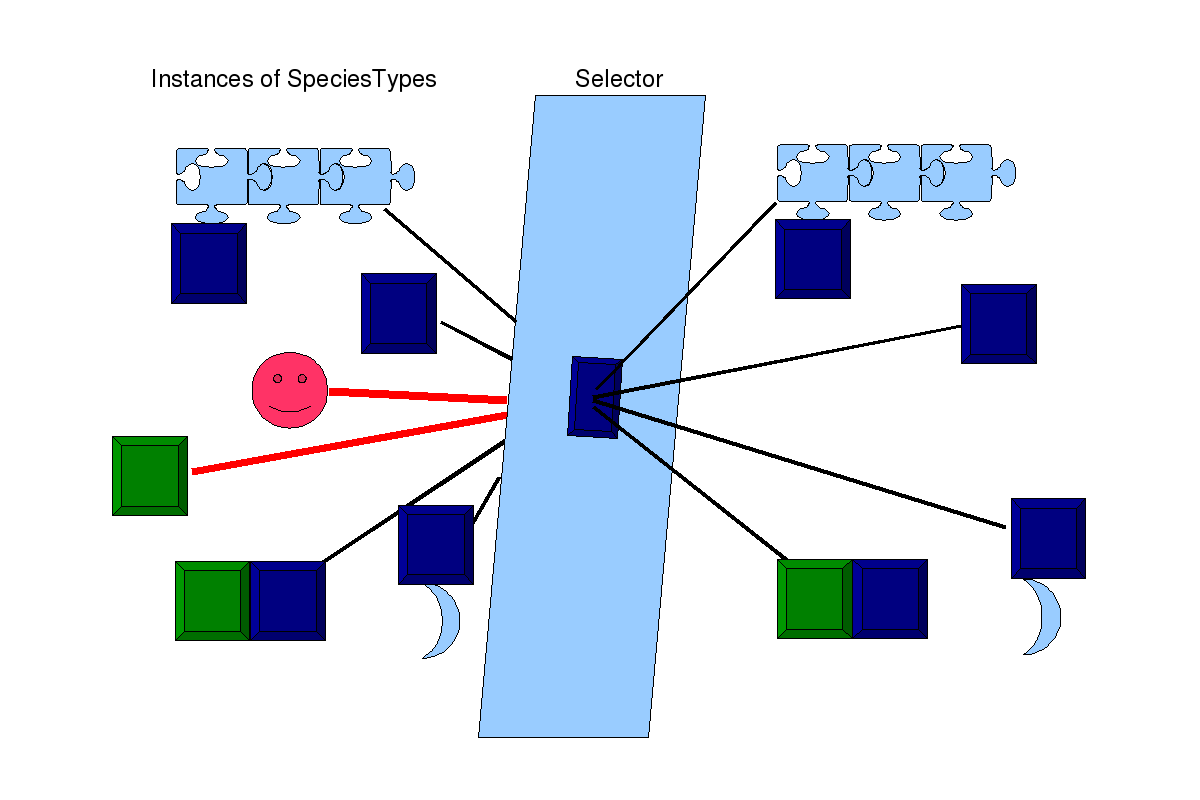
\includegraphics[scale=0.3]{figs/pngs/PrincipleIdeaSelector.png} 
\caption{The above selector accepts everything containing a blue crystal, but rejects the red face and the isolated green crystal.}
\label{fig:PrincipleIdeaSelector}
\end{center}
\end{figure}

A selector can be reused in various places of a model, to restrict the application of a procedure to a certain set of topologies and states. Selectors can be used to refine the initial conditions of a species, for instance to specify the initial distribution of different states and topologies. They can also be used in a reaction to decide if a this reaction happens, or to modulate its velocity, in function of the state or topology of a reactant. 

A selector defines the list of components composing the mask, that are species type existing under a given state (that can be an ensemble of elementary states). In addition to the components, the selector lists the possible or mandatory bonds, as well as the components that must not be bound. It is to be noted that a selector must not necessarily be the most parsimonious. One can use the selectors to describe the fine-grained topology of complexes, even if this topology is not used to decide upon particular reactions. The general structure of the selector is provided in \fig{SelectorGeneral} and the general structure of the species type state is provided in \fig{SpeciesTypeStateGeneral}.

\begin{figure}[H]
\begin{center}
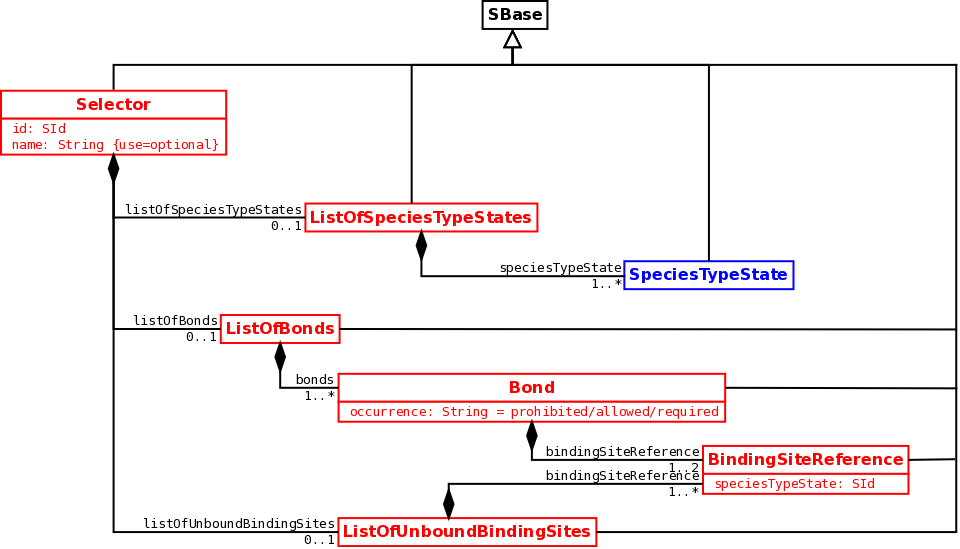
\includegraphics[scale=0.3]{figs/pngs/SelectorGeneral.png} 
\caption{\class{Selector} and all the associated classes.}
\label{fig:SelectorGeneral}
\end{center}
\end{figure}


\begin{figure}[H]
\begin{center}
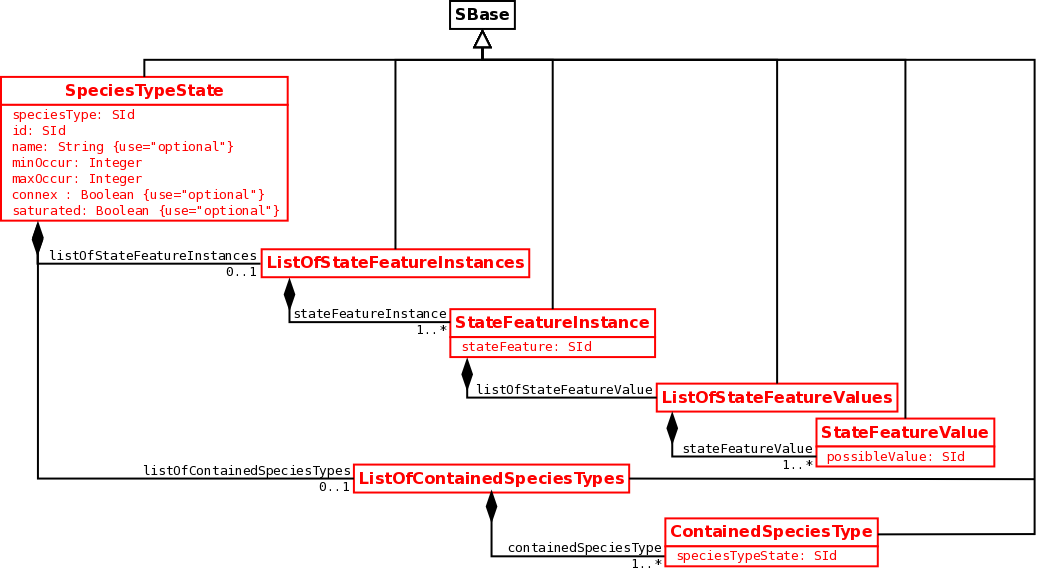
\includegraphics[scale=0.25]{figs/pngs/SpeciesTypeStateGeneral.png} 
\caption{\class{SpeciesTypeState} and all the associated classes.}
\label{fig:SpeciesTypeStateGeneral}
\end{center}
\end{figure}

A graphical representation of how to build a selector to encode a complex entity is represented on \fig{selectorBuilding}.

\begin{figure}[H]
\begin{center}
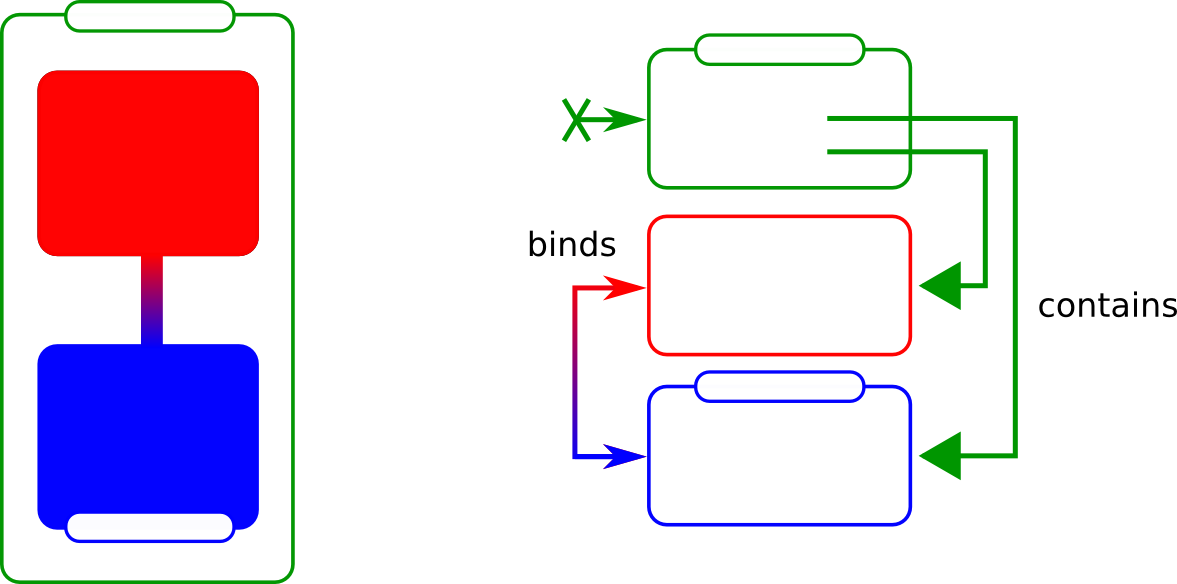
\includegraphics[scale=0.5]{figs/pngs/selectorBuilding.png}
\caption{This figure illustrates the procedure by which a selector builds the representation of a multi-state, multi-component complex. To encode the left part, representing the complex following the conventions used in this document, we write part represented on the right, listing the different components and their relationships.}
\label{fig:selectorBuilding}
\end{center}
\end{figure}

The \attribute{id} of \class{SpeciesTypeState} belong to a namespace local to the containing selector. Therefore, one can use the same values for \attribute{id} of \class{SpeciesTypeState} in different selectors. However, within a selector, all the values for \attribute{id} of \class{SpeciesTypeState} must be different.

\subsection{Selector}

A \class{Selector} is identified by an \attribute{id} and an optional \attribute{name}. As all elements derived from \class{SBase}, it can link to \class{Notes} and \class{Annotation}, and carry a \attribute{metaid}, and an \attribute{sboTerm}. In addition, a \class{Selector} is linked to a list of \class{SpeciesTypeState}s, a list of \class{Bond}s and  a list of  \class{BindingSiteReference}s.

\begin{figure}[H]
\begin{center}
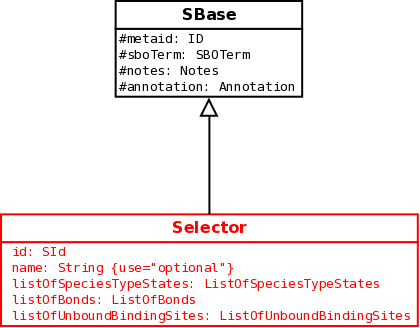
\includegraphics[scale=0.3]{figs/pngs/SelectorClass.png} 
\caption{Definition of \class{Selector} and its relation with \class{SBase}.}
\label{fig:SelectorClass}
\end{center}
\end{figure}

\begin{example}
<multi:selector 
                xmlns:multi="http://www.sbml.org/sbml/level3/version1/multi/version1" 
                multi:id="selector1"
                multi:name="unbound_receptor">
  <multi:listOfSpeciesTypeStates>
    <!-- some species type state -->
  </multi:listOfSpeciesTypeStates>
  <multi:listOfBonds>
    <!-- some bonds -->
  </multi:listOfBonds>
  <multi:listOfUnboundBindingSites>
    <!-- some unbound binding sites -->
  </multi:listOfUnboundBindingSites>
</multi:selector>
\end{example}

\subsection{SpeciesTypeState}

A species type state describes an ensemble of instances of a species type can be into, in order to fulfill the requirements of the selector. In order to build complex multi-component species, an instance of a species type can contain other instances of species types, that have to be declared in the selector also, with their allowed states. A species type state is then defined by the values of the different state features carried by the species type, the list of species type states it "contains", and their topology.
A \class{SpeciesTypeState} is identified by an \attribute{id} and an optional \attribute{name} plus an attribute \attribute{speciesType}, pointing to the \class{SpeciesType} it instantiates. As all elements derived from \class{SBase}, it can link to \class{Notes} and \class{Annotation}, and carry a \attribute{metaid}, and an \attribute{sboTerm}. In addition, a \class{SpeciesTypeState} can be linked to a list of \class{StateFeatureInstance}s and a list of \class{ContainedSpeciesType}s. A \class{SpeciesTypeState} can be instantiated several times in a selector, using the attributes \attribute{minOccur} and \attribute{maxOccur}. The attribute \attribute{connex} precises that all those instances must be part of a continuous network through bonds formed by the \class{ContainedSpeciesType}s. The attribute \attribute{saturated} precises that all \class{ContainedSpeciesType}s that are instances of \class{SpeciesType} with their attribute \attribute{bindingSite} set to true must be involved in bonds. 

\begin{figure}[H]
\begin{center}
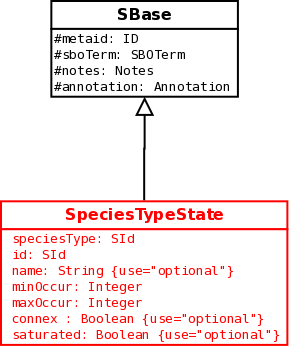
\includegraphics[scale=0.3]{figs/pngs/SpeciesTypeStateClass.png} 
\caption{Definition of \class{SpeciesTypeState} and its relation with \class{SBase}.}
\label{fig:SpeciesTypeStateClass}
\end{center}
\end{figure}

\begin{example}
<multi:speciesTypeState 
                    xmlns:multi="http://www.sbml.org/sbml/level3/version1/multi/version1" 
                    multi:id="speciesTypeState1" multi:name="open_receptor"
                    multi:speciesType="speciesType1"
                    multi:minOccur="2" multi:maxOccur="4"
                    multi:connex="true" multi:saturated="true" >
  <multi:listOfStateFeatureInstances>
    <!-- some state feature instances -->
  </multi:listOfStateFeatureInstances>
  <multi:listOfContainedSpeciesTypes>
    <!-- some contained species types -->
  </multi:listOfContainedSpeciesTypes>
</multi:speciesTypeState>
\end{example}

\subsection{StateFeatureInstance}

The possible states of an instance of species type are described using the state features of that species type. Only the meaningful state features, that are used to specified the state, must be listed. The other are assumed to take any value, to be wildcards. A  \class{StateFeatureInstance} is identified by an attribute \attribute{StateFeature}, pointing to the \class{StateFeature} it instantiates. As all elements derived from \class{SBase}, it can link to \class{Notes} and \class{Annotation}, and carry a \attribute{metaid}, and an \attribute{sboTerm}. In addition, a \class{StateFeatureInstance} can be linked to a list of \class{StateFeatureValue}s.

\begin{figure}[H]
\begin{center}
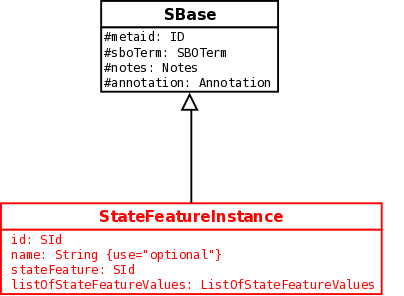
\includegraphics[scale=0.5]{figs/pngs/StateFeatureInstanceClass.png} 
\caption{Definition of \class{StateFeatureInstance} and its relation with \class{SBase}.}
\label{fig:StateFeatureInstanceClass}
\end{center}
\end{figure}

\begin{example}
<multi:stateFeatureInstance 
                    xmlns:multi="http://www.sbml.org/sbml/level3/version1/multi/version1" 
                    multi:stateFeature="stateFeature1">
  <!-- some state feature values -->
</multi:stateFeatureInstance>
\end{example}

\subsection{StateFeatureValue}

The selector specifies the values that a state feature of an instance of species type can take. A  \class{StateFeatureValue} points to the relevant \class{PossibleValue}s defined in the instantiated \class{SpeciesTypes} using an attribute \attribute{possibleValue}. As all elements derived from \class{SBase}, \class{StateFeatureValue} can link to \class{Notes} and \class{Annotation}, and carry a \attribute{metaid}, and an \attribute{sboTerm}.

\begin{figure}[H]
\begin{center}
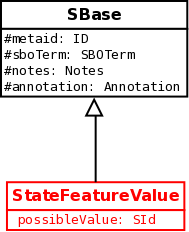
\includegraphics[scale=0.3]{figs/pngs/StateFeatureValueClass.png} 
\caption{Definition of \class{StateFeatureValue} and its relation with \class{SBase}.}
\label{fig:StateFeatureValueClass}
\end{center}
\end{figure}

\begin{example}
<multi:stateFeatureValue 
                    xmlns:multi="http://www.sbml.org/sbml/level3/version1/multi/version1" 
                    multi:possibleValue="possibleValue1" />
\end{example}

\subsection{ContainedSpeciesType}

In order to build complex nested multi-component species, an instance of a species type can contain other instances of species types, that have to be declared in the same selector. As all elements derived from \class{SBase}, \class{ContainedSpeciesType} can link to \class{Notes} and \class{Annotation}, and carry a \attribute{metaid}, and an \attribute{sboTerm}. In addition, a \class{ContainedSpeciesType} points to the relevant \class{SpeciesTypeState} using an attribute \attribute{speciesTypeState}. 

\begin{figure}[H]
\begin{center}
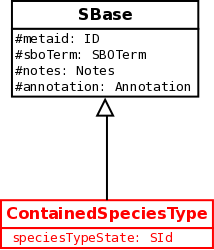
\includegraphics[scale=0.3]{figs/pngs/ContainedSpeciesTypeClass.png} 
\caption{Definition of \class{ContainedSpeciesType} and its relation with \class{SBase}.}
\label{fig:ContainedSpeciesTypeClass}
\end{center}
\end{figure}

\begin{example}
<multi:containedSpeciesType 
             xmlns:multi="http://www.sbml.org/sbml/level3/version1/multi/version1" 
             multi:speciesTypeState="speciesType1" />
\end{example}

\subsection{Bond}

The connectivity between the components of a selector is described by listing the bonds that are possible, mandatory or forbidden. As all elements derived from \class{SBase}, \class{Bond} can link to \class{Notes} and \class{Annotation}, and carry a \attribute{metaid}, and an \attribute{sboTerm}. An attribute \attribute{occurrence} specifies if a bond is \cdata{required}, \cdata{allowed} or \cdata{prohibited}. In addition, a \class{Bond} can be linked to a one or two \class{BindingReference}s.

\begin{figure}[H]
\begin{center}
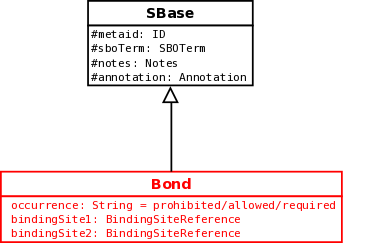
\includegraphics[scale=0.5]{figs/pngs/BondClass.png} 
\caption{Definition of \class{Bond} and its relation with \class{SBase}.}
\label{fig:BondClass}
\end{center}
\end{figure}

\begin{example}
<multi:bond xmlns:multi="http://www.sbml.org/sbml/level3/version1/multi/version1" 
            multi:occurrence="required" />
  <!-- some binding site references -->
</multi:bond>
\end{example}

\subsection{BindingSiteReference}

A component involved in a bond is specified by a \class{BindingSiteReference}. As all elements derived from \class{SBase}, it can link to \class{Notes} and \class{Annotation}, and carry a \attribute{metaid}, and an \attribute{sboTerm}. In addition, a \class{BindingSiteReference} refers to the component involved in the bond through the attribute \attribute{speciesTypeState}, that points to the value of the \attribute{id} attribute of the relevant \class{SpeciesTypeState}.

\begin{figure}[H]
\begin{center}
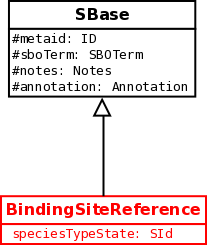
\includegraphics[scale=0.3]{figs/pngs/BindingSiteReferenceClass.png} 
\caption{Definition of \class{BindingSiteReference} and its relation with \class{SBase}.}
\label{fig:BindingSiteReferenceClass}
\end{center}
\end{figure}

\begin{example}
<multi:bindingSiteReference 
                    xmlns:multi="http://www.sbml.org/sbml/level3/version1/multi/version1" 
                    multi:speciesTypeState="speciesTypeState1" />
\end{example}

\subsection{Defining the components and the states allowed by the selector}

The following code contains a portion of selector describing two species type states, \cdata{speciesTypeState1} and \cdata{speciesTypeState2}. \cdata{SpeciesTypeState1} has a feature \cdata{stateFeature1} that can take the values \cdata{possibleValue1} or \cdata{possibleValue2} to pass the selection. In addition \cdata{speciesTypeState2} contains 4 instances of \cdata{speciesType2} (more exactly, it can contain between 4 and 4  instances of \cdata{speciesTypeState2} \ldots). The boolean attributes \attribute{connex} and \attribute{saturated} are of no use in this particular example, but are to be interpreted in conjunction with the bond definitions. 

\begin{example}
<multi:listOfSpeciesTypeStates
                  xmlns:multi="http://www.sbml.org/sbml/level3/version1/multi/version1">
  <multi:speciesTypeState multi:id="speciesTypeState1" multi:speciesType="speciesType1" 
                          multi:minOccur="4" multi:maxOccur="4" 
                          multi:connex="true" multi:saturated="true">
    <multi:listOfStateFeatureInstances>
      <multi:stateFeatureInstance multi:stateFeature="stateFeature1">
        <multi:listOfStateFeatureValues>
          <multi:stateFeatureValue multi:possibleValue="possibleValue1" />
          <multi:stateFeatureValue multi:possibleValue="possibleValue2" />
        </multi:listOfStateFeatureValues>
      </multi:stateFeatureInstance>
    </multi:listOfStateFeatureInstances>
  </multi:speciesTypeState>
  <multi:speciesTypeState multi:id="speciesTypeState2" multi:speciesType="speciesType2"
                          multi:minOccur="1" multi:maxOccur="1">
    <multi:listOfContainedSpeciesTypes>
      <multi:containedSpeciesType multi:speciesTypeState="speciesTypeState1" />
    </multi:listOfContainedSpeciesTypes>
  </multi:speciesTypeState>
</multi:listOfSpeciesTypeStates>
\end{example}

\begin{figure}[H]
\begin{center}
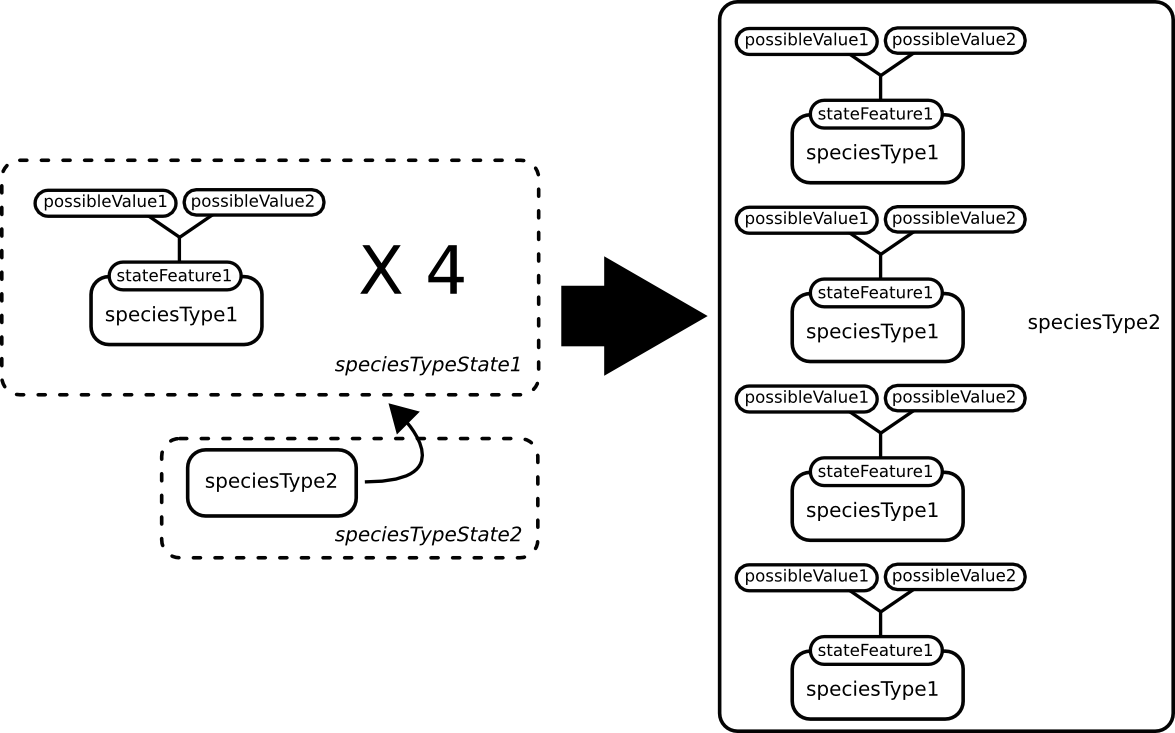
\includegraphics[scale=0.7]{figs/pngs/ex_sts.png} 
\caption{Generation of a nested selector from the definition of the two species type states, and the containment of one by the other.}
\label{fig:ex_sts}
\end{center}
\end{figure}

It is up to the model designer to avoid impossible structures, such as a species type state 1 that contains a species type 2, 2 itself containing 1. The following example is forbidden.

\color{red}
\begin{example}
<multi:listOfSpeciesTypeStates
                  xmlns:multi="http://www.sbml.org/sbml/level3/version1/multi/version1">
  <multi:speciesTypeState multi:id="speciesTypeState1" multi:speciesType="speciesType1" 
                          multi:minOccur="1" multi:maxOccur="1" >
    <multi:listOfContainedSpeciesTypes>
      <multi:containedSpeciesType multi:speciesTypeState="speciesTypeState2" />
    </multi:listOfContainedSpeciesTypes>
  </multi:speciesTypeState>
  <multi:speciesTypeState multi:id="speciesTypeState2" multi:speciesType="speciesType2"
                          multi:minOccur="1" multi:maxOccur="1" >
    <multi:listOfContainedSpeciesTypes>
      <multi:containedSpeciesType multi:speciesTypeState="speciesTypeState1" />
    </multi:listOfContainedSpeciesTypes>
  </multi:speciesTypeState>
</multi:listOfSpeciesTypeStates>
\end{example}
\normalcolor

If a species type is used in two different contexts, requiring for instance different numbers of occurrences,  two different species type states must be defined. For instance, if a species type A is used on its own in a species type C, or as contained twice in another species type B itself in C,  we need one A with min/maxOccur=1 and one A with min/maxOccur=2.

\begin{example}
<multi:listOfSpeciesTypeStates xmlns:multi="http://www.sbml.org/sbml/level3/version1/multi/version1">
  <multi:speciesTypeState multi:id="speciesTypeStateA1" multi:speciesType="speciesTypeA" 
                          multi:minOccur="1" multi:maxOccur="1" />
  <multi:speciesTypeState multi:id="speciesTypeStateA2" multi:speciesType="speciesTypeA"
                          multi:minOccur="2" multi:maxOccur="2" />
  <multi:speciesTypeState multi:id="speciesTypeStateB" multi:speciesType="speciesTypeB"
                          multi:minOccur="1" multi:maxOccur="1">
    <multi:listOfContainedSpeciesTypes>
      <multi:containedSpeciesType multi:speciesTypeState="speciesTypeStateA2" />
    </multi:listOfContainedSpeciesTypes>
  </multi:speciesTypeState>
  <multi:speciesTypeState multi:id="speciesTypeStateC" multi:speciesType="speciesTypeC"
                          multi:minOccur="1" multi:maxOccur="1" >
    <multi:listOfContainedSpeciesTypes>
      <multi:containedSpeciesType multi:speciesTypeState="speciesTypeStateA1" />
      <multi:containedSpeciesType multi:speciesTypeState="speciesTypeStateB" />
    </multi:listOfContainedSpeciesTypes>
  </multi:speciesTypeState>
</multi:listOfSpeciesTypeStates>
\end{example}

\begin{figure}[H]
\begin{center}
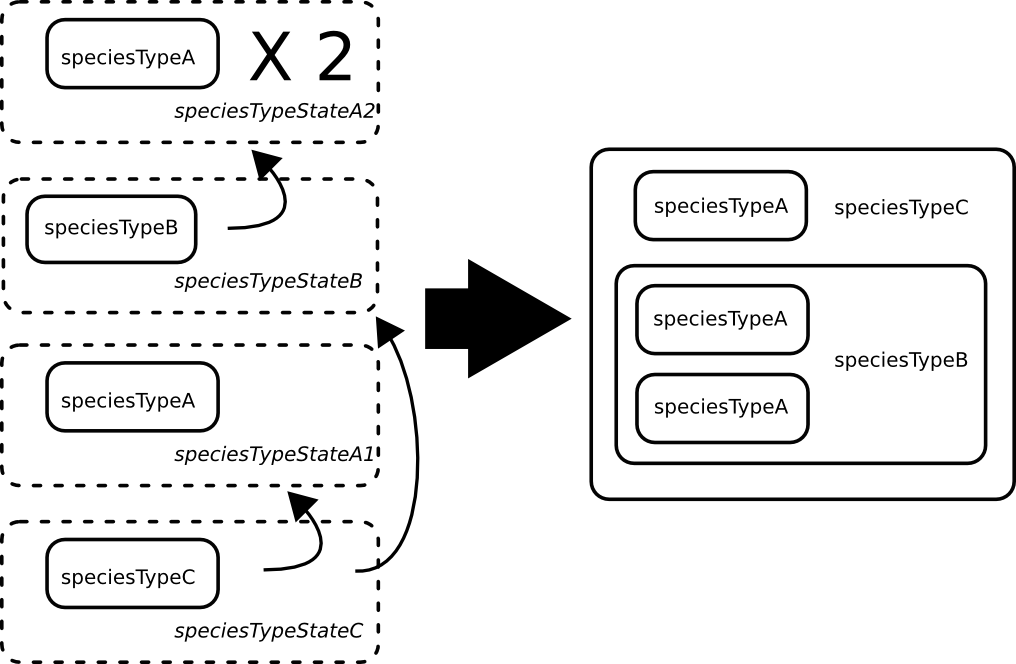
\includegraphics[scale=0.7]{figs/pngs/ex_sts_multiple.png} 
\caption{Nested selector where a given species type is used in two different contexts.}
\label{fig:ex_sts_multiple}
\end{center}
\end{figure}

The same species type can also be declared several time with different state feature values. The following example depicts a species type B containing two instances of species type A with a state feature displaying alternative values. Although in both case, the species type states refer to the same species type, we need to declare them separately.

\begin{example}
<multi:listOfSpeciesTypeStates
                   xmlns:multi="http://www.sbml.org/sbml/level3/version1/multi/version1">
  <multi:speciesTypeState multi:id="speciesTypeStateA1" multi:speciesType="speciesTypeA" 
                          multi:minOccur="1" multi:maxOccur="1" 
    <multi:listOfStateFeatureInstances>
      <multi:stateFeatureInstance multi:stateFeature="stateFeature1">
        <multi:listOfStateFeatureValues>
          <multi:stateFeatureValue multi:possibleValue="possibleValue1" />
        </multi:listOfStateFeatureValues>
      </multi:stateFeatureInstance>
    </multi:listOfStateFeatureInstances>
  </multi:speciesTypeState>
  <multi:speciesTypeState multi:id="speciesTypeStateA2" multi:speciesType="speciesTypeA" 
                          multi:minOccur="1" multi:maxOccur="1" 
    <multi:listOfStateFeatureInstances>
      <multi:stateFeatureInstance multi:stateFeature="stateFeature1">
        <multi:listOfStateFeatureValues>
          <multi:stateFeatureValue multi:possibleValue="possibleValue2" />
        </multi:listOfStateFeatureValues>
      </multi:stateFeatureInstance>
    </multi:listOfStateFeatureInstances>
  </multi:speciesTypeState>
  <multi:speciesTypeState multi:id="speciesTypeStateB" multi:speciesType="speciesTypeB"
                          multi:minOccur="1" multi:maxOccur="1">
    <multi:listOfContainedSpeciesTypes>
      <multi:containedSpeciesType multi:speciesTypeState="speciesTypeStateA1" />
      <multi:containedSpeciesType multi:speciesTypeState="speciesTypeStateA2" />
    </multi:listOfContainedSpeciesTypes>
  </multi:speciesTypeState>
</multi:listOfSpeciesTypeStates>
\end{example}

\begin{figure}[H]
\begin{center}
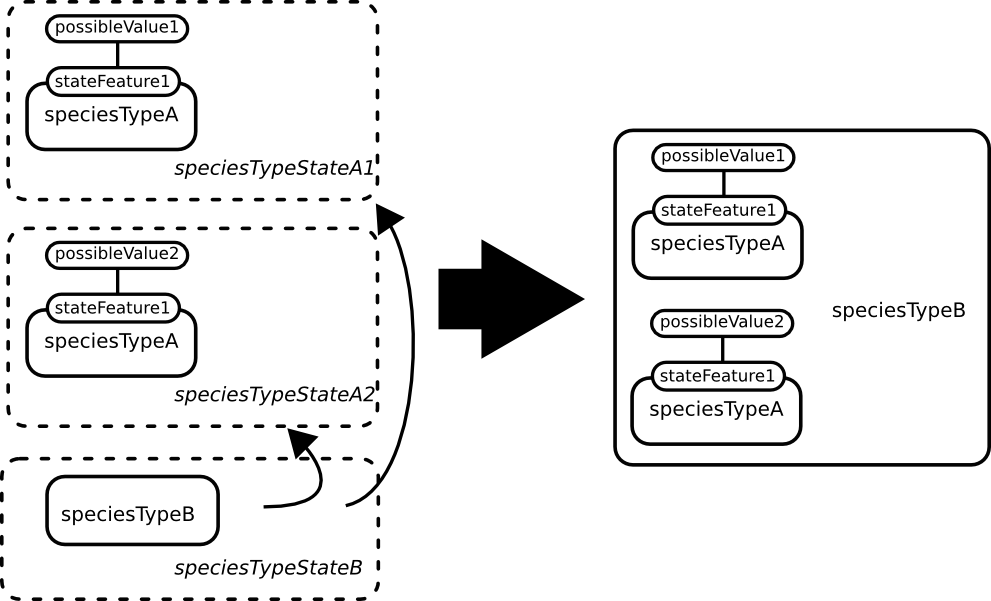
\includegraphics[scale=0.7]{figs/pngs/ex_sts_differentStates.png} 
\caption{Nested selector where a given species type is used with two different state feature values.}
\label{fig:ex_sts_differentStates}
\end{center}
\end{figure}

\subsection{Defining the connectivities allowed by the selector}
 
In a selector, instances of species types possessing an attribute \attribute{bindingSite} set to \cdata{true} can be referred to when they are involved in bonds, or explicitly listed as unbound. As a result such a species type can be used in four different contexts:

\begin{itemize}
 \item In a declared explicit bond, with another specific instance of a species type (represented by a bond linking two black entities in the example graphs). 

\begin{example}
<multi:bond xmlns:multi="http://www.sbml.org/sbml/level3/version1/multi/version1" 
            multi:occurrence="required" >
  <multi:bindingSiteReference multi:speciesTypeState="speciesTypeState1" />
  <multi:bindingSiteReference multi:speciesTypeState="speciesTypeState2" />
</multi:bond>
\end{example}

 \item In a declared generic bond without another specific instance of a species type (represented by an unlinked black entity in the example graphs). 

\begin{example}
<multi:bond xmlns:multi="http://www.sbml.org/sbml/level3/version1/multi/version1" 
            multi:occurrence="required" >
  <multi:bindingSiteReference multi:speciesTypeState="speciesTypeState1" />
</multi:bond>
\end{example}

 \item Declared as explicitly unbound (represented by a white entity in the example graphs). 

\begin{example}
<multi:listOfUnboundBindingSites 
             xmlns:multi="http://www.sbml.org/sbml/level3/version1/multi/version1" />
  <multi:bindingSiteReference multi:speciesTypeState="speciesTypeState1" />
</multi:listOfUnboundBindingSites>
\end{example}

\item Undeclared, meaning that one does not care if it is bound or not (represented by a gray entity in the example graphs). 
\end{itemize}

A given binding site can only be bound to another binding site. If three instances of species types are bound together, they have to be bound through different contained binding sites. Those binding sites can be different instances of the same species type (``identical'' binding sites) or instances of different species types (different binding sites). The following example is forbidden:

\color{red}
\begin{example}
<multi:listOfBonds xmlns:multi="http://www.sbml.org/sbml/level3/version1/multi/version1">
  <multi:bond multi:occurrence="required" >
    <multi:bindingSiteReference multi:speciesTypeState="speciesTypeStateA" />
    <multi:bindingSiteReference multi:speciesTypeState="speciesTypeStateB" />
  </multi:bond>
  <multi:bond multi:occurrence="required" >
    <multi:bindingSiteReference multi:speciesTypeState="speciesTypeStateA" />
    <multi:bindingSiteReference multi:speciesTypeState="speciesTypeStateC" />
  </multi:bond>
</multi:listOfBonds>
\end{example}
\normalcolor

Instead the following code should be used, where \cdata{speciesTypeStateA1} and \cdata{speciesTypeStateA2} are two different species type states of the same species type.

\color{blue}
\begin{example}
<multi:listOfBonds xmlns:multi="http://www.sbml.org/sbml/level3/version1/multi/version1">
  <multi:bond multi:occurrence="required" >
    <multi:bindingSiteReference multi:speciesTypeState="speciesTypeStateA1" />
    <multi:bindingSiteReference multi:speciesTypeState="speciesTypeStateB" />
  </multi:bond>
  <multi:bond multi:occurrence="required" >
    <multi:bindingSiteReference multi:speciesTypeState="speciesTypeStateA2" />
    <multi:bindingSiteReference multi:speciesTypeState="speciesTypeStateC" />
  </multi:bond>
</multi:listOfBonds>
\end{example}
\normalcolor

\begin{figure}[H]
\begin{center}
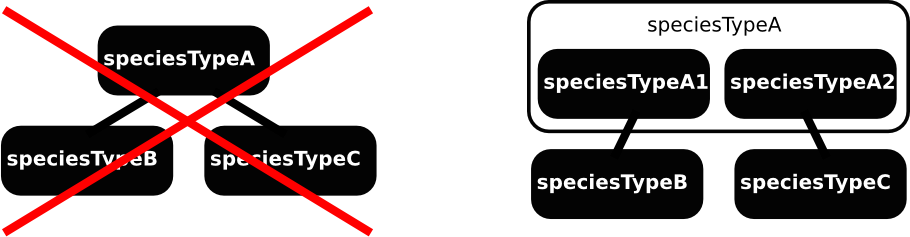
\includegraphics[scale=0.7]{figs/pngs/ex_multipleBinding.png} 
\caption{The connectivity on the left is forbidden, and the connectivity on the right should be used instead.}
\label{fig:ex_multipleBinding}
\end{center}
\end{figure}

The description of the connectivity through the list of bonds and the list of unbound binding sites is greedy. In other words, the possible connectivity is the sum of all the different listed possibilities. If in a selector, an instance of a species type is involved in at least one allowed bond, then it must be bound to something. It cannot be unbound. Furthermore, if an instance of a species type is involved in listed bonds, only the listed bonds can fulfill the selection. 

The attribute \attribute{occurrence}, in combination with explicit, generic and undeclared bonds, provides for a complete boolean logic to select the context of bindingSites. Note that \attribute{occurrence} is only present on \class{Bond}. In order to forbid a binding site to be unbound, we create a generic bond with \attribute{occurrence} set to \cdata{required} (to say that X cannot be free is equivalent to say that X had to be bound to something, whatever it is).

To exemplify this boolean logic, let's take the example of an instance of a species type X interacting with instances of species type A, B or C.

In the following code, X is not declared at all, therefore X can be bound to A, B, C or be unbound:

\begin{example}
<multi:selector xmlns:multi="http://www.sbml.org/sbml/level3/version1/multi/version1" 
                multi:id="selector1" />
  <multi:listOfSpeciesTypeStates>
    <multi:speciesTypeState id="speciesTypeStateA" speciesType="speciesTypeA"                                           
                            multi:minOccur="1" multi:maxOccur="1" />
    <multi:speciesTypeState id="speciesTypeStateB" speciesType="speciesTypeB"                           
                            multi:minOccur="1" multi:maxOccur="1" />
  </multi:listOfSpeciesTypeStates>
</multi:selector> 
\end{example}

With the following code, X can only be bound to A, or unbound:

\begin{example}
<multi:selector xmlns:multi="http://www.sbml.org/sbml/level3/version1/multi/version1" 
                multi:id="selector1" />
  <multi:listOfSpeciesTypeStates>
    <multi:speciesTypeState id="speciesTypeStateX" speciesType="speciesTypeX"                                           
                            multi:minOccur="1" multi:maxOccur="1" />
    <multi:speciesTypeState id="speciesTypeStateA" speciesType="speciesTypeA"                           
                            multi:minOccur="1" multi:maxOccur="1" />
  </multi:listOfSpeciesTypeStates>
  <multi:listOfBonds xmlns:multi="http://www.sbml.org/sbml/level3/version1/multi/version1" >
    <multi:bond multi:occurrence="allowed" >
      <multi:bindingSiteReference multi:speciesTypeState="speciesTypeStateX" />
      <multi:bindingSiteReference multi:speciesTypeState="speciesTypeStateA" />
    </multi:bond>
  </multi:listOfBonds>
</multi:selector> 
\end{example}

With the following code X can only be bound either to A or B, but not C:

\begin{example}
<multi:selector xmlns:multi="http://www.sbml.org/sbml/level3/version1/multi/version1" 
                multi:id="selector1" />
  <multi:listOfSpeciesTypeStates>
    <multi:speciesTypeState id="speciesTypeStateX" speciesType="speciesTypeX"                                           
                            multi:minOccur="1" multi:maxOccur="1" />
    <multi:speciesTypeState id="speciesTypeStateA" speciesType="speciesTypeA"                           
                            multi:minOccur="1" multi:maxOccur="1" />
    <multi:speciesTypeState id="speciesTypeStateB" speciesType="speciesTypeB"                           
                            multi:minOccur="1" multi:maxOccur="1" />
  </multi:listOfSpeciesTypeStates>
  <multi:listOfBonds xmlns:multi="http://www.sbml.org/sbml/level3/version1/multi/version1">
    <multi:bond multi:occurrence="allowed" >
      <multi:bindingSiteReference multi:speciesTypeState="speciesTypeStateX" />
      <multi:bindingSiteReference multi:speciesTypeState="speciesTypeStateA" />
    </multi:bond>
    <multi:bond multi:occurrence="allowed" >
      <multi:bindingSiteReference multi:speciesTypeState="speciesTypeStateX" />
      <multi:bindingSiteReference multi:speciesTypeState="speciesTypeStateB" />
    </multi:bond>
  </multi:listOfBonds>
</multi:selector> 
\end{example}

The following code defines a generic bond with X, which mean that X can be bound to A, B or C, but has to be bound to something:

\begin{example}
<multi:selector xmlns:multi="http://www.sbml.org/sbml/level3/version1/multi/version1" 
                multi:id="selector1" />
  <multi:listOfSpeciesTypeStates>
    <multi:speciesTypeState id="speciesTypeStateX" speciesType="speciesTypeX"                                           
                            multi:minOccur="1" multi:maxOccur="1" />
  </multi:listOfSpeciesTypeStates>
  <multi:listOfBonds xmlns:multi="http://www.sbml.org/sbml/level3/version1/multi/version1" >
    <multi:bond multi:occurrence="allowed" >
      <multi:bindingSiteReference multi:speciesTypeState="speciesTypeStateX" />
    </multi:bond>
  </multi:listOfBonds>
</multi:selector> 
\end{example}

The following code says that X cannot be bound to C (The bond X-C is prohibited), and therefore has to be bound to A or B or unbound.

\begin{example}
<multi:selector xmlns:multi="http://www.sbml.org/sbml/level3/version1/multi/version1" 
                multi:id="selector1" />
  <multi:listOfSpeciesTypeStates>
    <multi:speciesTypeState id="speciesTypeStateX" speciesType="speciesTypeX"                                           
                            multi:minOccur="1" multi:maxOccur="1" />
    <multi:speciesTypeState id="speciesTypeStateC" speciesType="speciesTypeC"                           
                            multi:minOccur="1" multi:maxOccur="1" />
  </multi:listOfSpeciesTypeStates>
  <multi:listOfBonds xmlns:multi="http://www.sbml.org/sbml/level3/version1/multi/version1">
    <multi:bond multi:occurrence="prohibited" >
      <multi:bindingSiteReference multi:speciesTypeState="speciesTypeStateX" />
      <multi:bindingSiteReference multi:speciesTypeState="speciesTypeStateC" />
    </multi:bond>
  </multi:listOfBonds>
</multi:selector> 
\end{example}
 
The following code says that X cannot be bound to C (The bond X-C is prohibited), however a generic bond specifies that X has to bound to something, therefore effectively to A or B. In this particular example, \attribute{occurrence} on the generic bond can be set indifferently to \cdata{allowed} or \cdata{required}.

\begin{example}
<multi:selector xmlns:multi="http://www.sbml.org/sbml/level3/version1/multi/version1" 
                multi:id="selector1" />
  <multi:listOfSpeciesTypeStates>
    <multi:speciesTypeState id="speciesTypeStateX" speciesType="speciesTypeX"                                           
                            multi:minOccur="1" multi:maxOccur="1" />
    <multi:speciesTypeState id="speciesTypeStateC" speciesType="speciesTypeC"                           
                            multi:minOccur="1" multi:maxOccur="1" />
  </multi:listOfSpeciesTypeStates>
  <multi:listOfBonds xmlns:multi="http://www.sbml.org/sbml/level3/version1/multi/version1" >
    <multi:bond multi:occurrence="prohibited" >
      <multi:bindingSiteReference multi:speciesTypeState="speciesTypeStateX" />
      <multi:bindingSiteReference multi:speciesTypeState="speciesTypeStateC" />
    </multi:bond>
    <multi:bond multi:occurrence="allowed" >
      <multi:bindingSiteReference multi:speciesTypeState="speciesTypeStateX" />
    </multi:bond>
  </multi:listOfBonds>
</multi:selector> 
\end{example}

The following case is overdetermined, since the impossibility for X to bind C is implicit in the restriction of its binding to A or B.

\begin{example}
<multi:selector xmlns:multi="http://www.sbml.org/sbml/level3/version1/multi/version1" 
                multi:id="selector1" />
  <multi:listOfSpeciesTypeStates>
    <multi:speciesTypeState id="speciesTypeStateX" speciesType="speciesTypeX"                                           
                            multi:minOccur="1" multi:maxOccur="1" />
    <multi:speciesTypeState id="speciesTypeStateA" speciesType="speciesTypeA"                           
                            multi:minOccur="1" multi:maxOccur="1" />
    <multi:speciesTypeState id="speciesTypeStateB" speciesType="speciesTypeB"                           
                            multi:minOccur="1" multi:maxOccur="1" />
    <multi:speciesTypeState id="speciesTypeStateC" speciesType="speciesTypeC"                           
                            multi:minOccur="1" multi:maxOccur="1" />
  </multi:listOfSpeciesTypeStates>
  <multi:listOfBonds xmlns:multi="http://www.sbml.org/sbml/level3/version1/multi/version1">
    <multi:bond multi:occurrence="allowed" >
      <multi:bindingSiteReference multi:speciesTypeState="speciesTypeStateX" />
      <multi:bindingSiteReference multi:speciesTypeState="speciesTypeStateA" />
    </multi:bond>
    <multi:bond multi:occurrence="allowed" >
      <multi:bindingSiteReference multi:speciesTypeState="speciesTypeStateX" />
      <multi:bindingSiteReference multi:speciesTypeState="speciesTypeStateB" />
    </multi:bond>
    <multi:bond multi:occurrence="prohibited" >
      <multi:bindingSiteReference multi:speciesTypeState="speciesTypeStateX" />
      <multi:bindingSiteReference multi:speciesTypeState="speciesTypeStateC" />
    </multi:bond>
  </multi:listOfBonds>
</multi:selector> 
\end{example}

The boolean attributes \attribute{connex} and \attribute{saturated} precise the topology of a multimeric assembly of the same component (same species type state, that is same species type with the same values allowed for all their state features). One can then declare the component only once, and each of the bond types or unbound binding sites only once. Attribute \attribute{saturated} set to \cdata{true} means that all the contained species types which \attribute{bindingSite} is set to \cdata{true} have to be bound. Attribute \attribute{connex} means that all the instances of the species type state have to be connected within the same complex. The following example presents a tetramer of identical subunits. 

\begin{example}
<multi:selector xmlns:multi="http://www.sbml.org/sbml/level3/version1/multi/version1" 
                multi:id="selector1" />
  <multi:listOfSpeciesTypeStates>
    <multi:speciesTypeState id="speciesTypeStateA" speciesType="speciesTypeA"                                           
                            multi:minOccur="4" multi:maxOccur="4"
                            connex="{true|false}" saturated="{true|false}">
      <multi:listOfContainedSpeciesTypes>
        <multi:containedSpeciesType multi:speciesTypeState="speciesTypeStateB" />
        <multi:containedSpeciesType multi:speciesTypeState="speciesTypeStateC" />
      </multi:listOfContainedSpeciesTypes>
    </multi:speciesTypeState>
    <multi:speciesTypeState id="speciesTypeStateB" speciesType="speciesTypeB"                                           
                            multi:minOccur="1" multi:maxOccur="1" />
    <multi:speciesTypeState id="speciesTypeStateC" speciesType="speciesTypeC"                                           
                            multi:minOccur="1" multi:maxOccur="1" />
  </multi:listOfSpeciesTypeStates>
  <multi:listOfBonds xmlns:multi="http://www.sbml.org/sbml/level3/version1/multi/version1">
    <multi:bond multi:occurrence="allowed" >
      <multi:bindingSiteReference multi:speciesTypeState="speciesTypeStateB" />
      <multi:bindingSiteReference multi:speciesTypeState="speciesTypeStateC" />
    </multi:bond>
  </multi:listOfBonds>
</multi:selector> 
\end{example}

The following graphs are examples of the various combinations possible of \attribute{connex} and \attribute{saturated} attributes. 

\begin{figure}[H]
\begin{center}
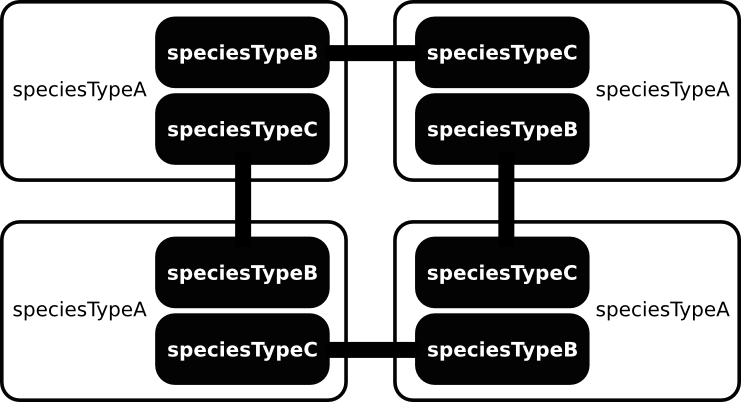
\includegraphics[scale=0.7]{figs/pngs/ex_connex-saturated.png} 
\caption{\xmlcode{connex="true" saturated="true"}}
\label{fig:ex_connex-saturated}
\end{center}
\end{figure}

\begin{figure}[H]
\begin{center}
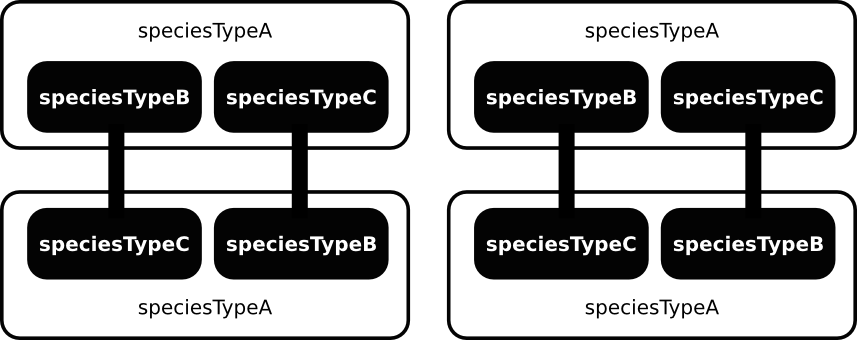
\includegraphics[scale=0.7]{figs/pngs/ex_nonconnex-saturated.png} 
\caption{\xmlcode{connex="false" saturated="true"}}
\label{fig:ex_nonconnex-saturated}
\end{center}
\end{figure}

\begin{figure}[H]
\begin{center}
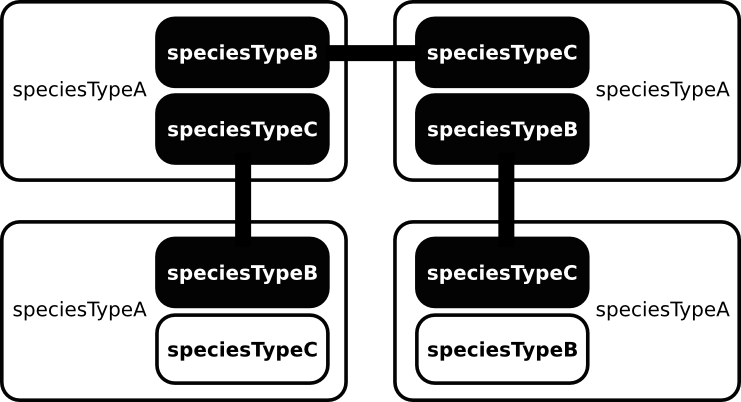
\includegraphics[scale=0.7]{figs/pngs/ex_connex-nonsaturated.png} 
\caption{\xmlcode{connex="true" saturated="false"}}
\label{fig:ex_connex-nonsaturated}
\end{center}
\end{figure}

\begin{figure}[H]
\begin{center}
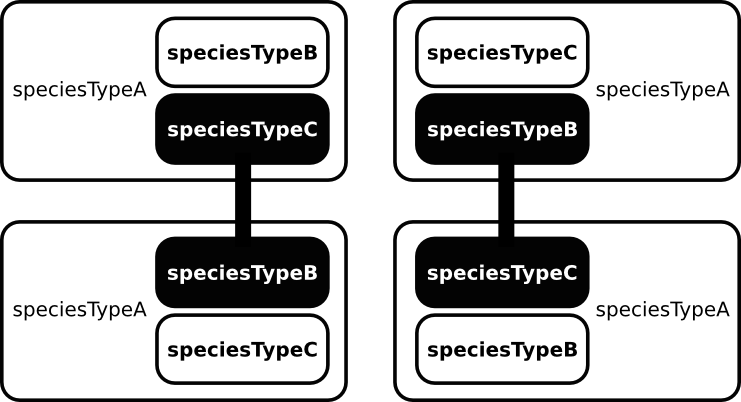
\includegraphics[scale=0.7]{figs/pngs/ex_nonconnex-nonsaturated.png} 
\caption{\xmlcode{connex="false" saturated="false"}}
\label{fig:ex_nonconnex-nonsaturated}
\end{center}
\end{figure}
